\documentclass{article}
\usepackage{graphicx} % Required for inserting images
\usepackage{amsmath}
\usepackage{amssymb}
\usepackage{url}
\usepackage{biblatex}
\usepackage{algorithm}
\usepackage{algorithmicx}
\usepackage{algpseudocode}


\addbibresource{refs.bib}
\title{SNA: Neural Net for Blokus}
\author{Ilmari Vahteristo, Zhi-Song Liu, Andreas Rupp}
\date{August 2024}

\begin{document}

\maketitle

\section{Introduction}
This document provides a brief description of what I did in the summer of 2024 to try and create a neural network player for the Blokus Classic board game. This is not a comprehensive description, nor necessarily written in an academic style. Rather, this document is a minimal description of what I did in the summer of 2024 to create a NN based Blokus player. It doesn't contain everything that was tried, but tries to collect the most interesting and surprising results, and what was learned from them.

\subsection{Reinforcement learning}
Reinforcement learning (RL) is a type of machine learning in which an agent learns to take actions in an environment by interacting with it. The agent receives numeric feedback (reward) through a reward function that gives positive/negative values relative to how good a position is. Often, the reward functions are sparse, meaning that the agent only rarely receives feedback about its sequence of actions. RL has many problems, such as sparse, delayed, or noisy signals and sample inefficiency.


Reinforcement learning has been extensively used in games, but relatively little in real-world applications. Humans can often overcome typical RL problems, since they have very strong prior knowledge about the world and how objects function. For example, Dubey et. al. show how human performance degrades in an Atari-type game when priors are mitigated \cite{dubey2018investigating}.



\subsection{Blokus}
Blokus Classic (just Blokus from now on) is a board game played between 4 players on a 20x20 board. Each player tries to occupy the most area from the board, using the same set of pieces. Additionally, being able to place all of your pieces gives +15, and placing your unit grid piece as your last piece gives a +5 score. The Blokus board and the pieces can be seen in Figure \ref{fig:blokus_board}.

\begin{figure}[h]
    \centering
    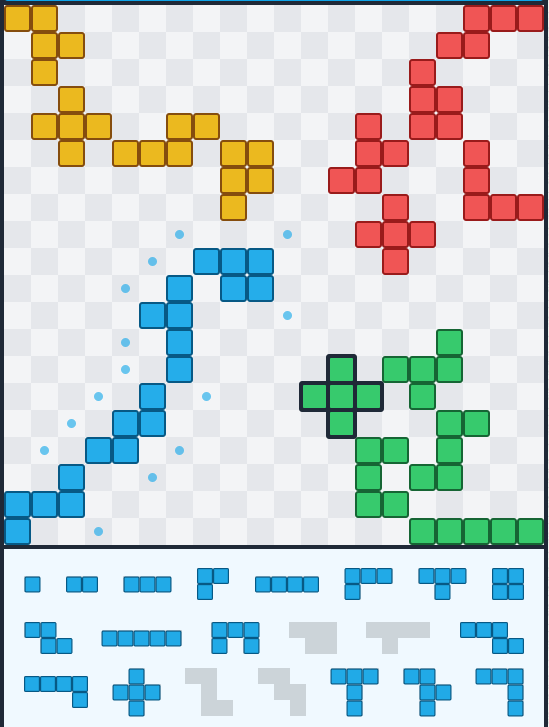
\includegraphics[width=0.4\linewidth]{blokus_board.png}
    \caption{A Blokus game in progress. Blue dots show all grids that don't share an edge, and share a corner with the existing blue pieces.}
    \label{fig:blokus_board}
\end{figure}


In the first move of the game, each player must place their first piece in a way that he covers his own corner grid. After the first move, you can place any of your piece, in any orientation, to any place where 1) The piece fits the board, i.e. doesn't overlap with any other piece, 2) Doesn't share an edge with the player's own piece, and 3) the placed piece shares atleast one corner with the player's own pieces. For examples of valid placements, see again Figure \ref{fig:blokus_board}.

\subsection{Software}
As a backend for Blokus, we use the Open source Pentobi \cite{Enzenberger2011Pentobi} computer program that provides the game logic, nine different players (levels 1-9, all using Monte-Carlo Tree search), and some developer tools. We write a wrapper for the Pentobi library, specifically for the Go Text Protocol (GTP) interface, that allows us to control a Blokus game through the command line (or Python in our case). Our Python wrapper can be found from GitHub \cite{Vahteristo2024PythonBlokus}.


\section{Methodology}

Our approach to learning to play Blokus is Simulation Neural Network Alternation (SNA). We experiment with various NN architectures, optimization parameters, and initial policies.

We create three different datasets, using three different agents to simulate the games: random play, or level 1, or level 5 Pentobi players. We use these datasets to test neural network architectures under fixed conditions. We then use the most promising architectures in the SNA simulations. More about data creation in \ref{}.

\subsection{Reinforcement learning}
This section will explain reinforcement learning more formally, and we will explain our notation.

\noindent Consider the following:
\begin{itemize}
\item A set of states $S$ describing all the possible states that the environment can be in.
\item A set of actions $A$ that contains all actions that can be taken in at least one state of the environment,
\item A subset $A_s \subseteq A$, that only contains the actions that are legal in state $s$,
\item A reward function $R: S\times A \rightarrow \mathbb{R}$ describing a numeric feedback from making action $a$ in state $s$, and
\item A transition function $T : S\times A \rightarrow S$ which calculates the next state $s_{t+1}$ after action $a$: $s_{t+1} = T(s_t,a)$. Note that this function $T$ is the transformation of the state to the next state \emph{in which the agent can take an action again}. Hence, in a multi-agent environment, the function $T$ also incorporates the decisions of other players.
\end{itemize}
The objective of reinforcement learning is to learn a policy $\pi : S \rightarrow A$ that maximizes the expected total cumulated reward over an episode:$$\sum_{t=0}^{t=\tau}R(s_t,\pi(s_t)),$$ where $s_{t+1}=T(s_t,\pi(s_t))$, and $\tau$ is the length of an episode ($s_\tau$ is a terminal state).

If one has a function $Q^{\pi} : S\times A \rightarrow \mathbb{R}$, that accurately estimates the expected cumulated reward obtained after an episode by making action $a$ in state $s$ and continuing with policy $\pi$ then the optimal policy $\pi^*$ will be to try each $a$ in $A_s$ and choose the one with the highest $Q$ value: $$\pi^{*}(s) = \arg\!\max_{a \in A_s} Q^\pi(s,a).$$

In some problems we have a model of the environment, meaning that we know the transition function $T$.
Knowing $T$ typically makes the problem easier, since $Q$ can be considered to be composed of $T$ and a value function $V^{\pi}(s) = E[P_\pi(r|s)]$ that tells the expected reward from playing with policy $\pi$ from the state $s$ to termination. The function $Q$ calculates how good the next state is after applying the transition T: $Q^{\pi}(s,a) = V^{\pi}(T(s,a))$. Hence, if $T$ is known, it is enough to learn the value function, which is easier due to the smaller input space.

Knowing $T$ also allows us to compensate for a poor value function by searching deeper than just one action ahead by using any tree search algorithm. A tree search allows us to look further into the future and avoid a 'horizon effect' \cite{marsland1991computer} where immediately good decisions are poor long-term.

In environments with an adversary, we do not know $T$ completely, since we do not know which action the adversary will take. Assuming that we know the state $s$ exactly and that we always know the subset of actions $A_s$ that the adversary can take, we sometimes assume that the adversary will try to maximize their score/value. Using this assumption we can consider $T$ known and search the tree using a tree search. This is known as Minimax search \cite{kiefer1953sequential}.

\subsection{SNA}

\label{SNA}
\begin{algorithm}
\caption{Basic SNA Algorithm}
\label{alg:q-sna}
\begin{algorithmic}[1]
\State Initialize policy $\pi_0$
\For{each iteration $i$ = $0...N$}
    \State Sample $P_{\pi_i}(r|s)$ with simulations
    \State Create an estimator $\hat{V}^{\pi_i}(s) \approx E[P_{\pi_i}(r|s)]$ using the simulated data
    \State Update the policy:
    \State $$\pi_{i+1}(s) =  \arg\!\max_{a \in A_s} \hat{V}^{\pi_i}(T(s,a))$$
\EndFor
\end{algorithmic}
\end{algorithm}
We start with some initial policy $\pi_0$, for example random play, or an existing policy. We sample $P_{\pi_i}(r|s)$, i.e. we simulate episodes in the environment where all players use the policy $\pi_i$ and record the observed $s,r$ pairs.
We then train a neural network to estimate the true value function using the $(r,s)$ pairs, i.e. $\hat{V}^{\pi_i}(s) = E[P_{\pi_i}(r|s)]$.
At the end of each iteration, we use $\hat{V}^{\pi_i}$ to create a new policy $\pi_{i+1}(s) = \arg\!\max_{a \in A_s} \hat{V}^{\pi_i}(T(s,a))$.
If we have an accurate estimator (NN converged, enough data, and NN capacity), we know the policy $\pi_{i+1}$ is a better policy than $\pi_{i}$.

This is a slightly simplified algorithm. In practice, the policy needs to have some amount of randomness/exploration, otherwise the estimator cannot learn new strategies. In our experiments, we use epsilon-greedy exploration with $\epsilon=0.1$.
Additionally, instead of only simulating episodes where all players use the same policy (+randomness), it is beneficial to sometimes use previous policies in the simulations. In our experiments we use previous policies weighted by how often the policy wins the initial policy $\pi_0$ in a four-player game. For the initial policy itself, $P(\text{"win against three } \pi_0 \text{" }| \pi_0) = 0.25$.

\subsection{Data and preprocessing}
\label{sec:data-prepocessing}
As data, we use state-reward pairs that we obtain from simulations. Each state consists of 402 values: The 20x20 flattened board, who is the next player to move, and which player's reward we are assessing.

While simulating, we record the state after a player has made a move. This means that the model will learn to evaluate how good the state is after we have made a move but will not learn to evaluate how good a state we were given is. For the SNA algorithm, we do not need to know how good the state we receive is - we just need to know how we should leave it. It might be easy to also learn to evaluate the state we are given, but it is certainly easier to not learn it.

Each grid in the board is -1 if it is empty, and otherwise 0,1,2, or 3 according to which player's piece is in it.
We save the data across multiple files and load the data in parallel from the files, with a non-deterministic order.

\subsubsection{Preprocessing}
\begin{figure}
    \centering
    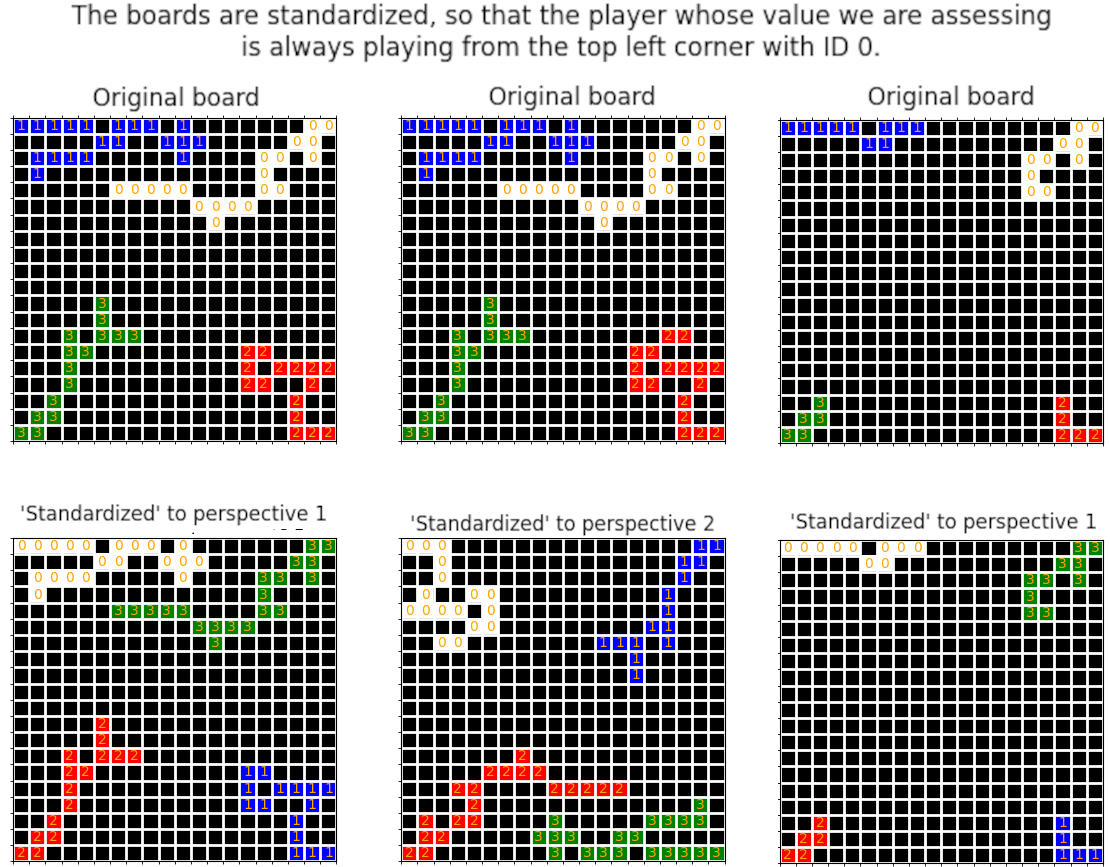
\includegraphics[width=1\linewidth]{blokus_std_boards_edited.png}
    \caption{Each Blokus board is standardized for the neural net input to reduce what the model has to learn.}
    \label{fig:blokus-board-std}
\end{figure}

To avoid data augmentations and avoid needing to learn rotational invariance etc., we standardize each sample as follows (Figure \ref{fig:blokus-board-std}):
\begin{itemize}
    \item Convert each grid (except empty grids) in the board so the player whose turn it is is marked as 0, the player after them is 1, etc.
    \item Rotate the 20x20 board, s.t. a grid with the value 0 is in the top left corner.
\end{itemize}
This transformation ensures that the model gives the same estimate for each player in the same position. We do this transformation online, during inference.

Each label is a one-hot encoded vector of the obtained rank (rank vector). The total reward is the dot product of the rank vector and the weights $[3,2,1,0]$. Hence, a win is 3 points, second position is 2, third is 1, and last place is 0.

\subsubsection{Gathering datasets}
\label{sec:gathering-datasets}
We create three different datasets to evaluate different NN architectures under the same conditions. We keep the simulation settings the same, except that we change the player policy. In all datasets, we simulate 2 million games, and with non-random play (D1 and D5), we use an epsilon-greedy exploration with $\epsilon=0.1$.
The datasets are:
\begin{itemize}
    \item (D0) In this dataset the player play entirely randomly.
    \item (D1) This dataset uses level 1 Pentobi players.
    \item (D5) This dataset uses level 5 Pentobi players.
\end{itemize}

\noindent Each game yields about 60 labeled states, so each dataset has about 120 million labeled states in total. For reference, Deepmind used a dataset of 10 million human Chess games (15 billion labeled states) to train their neural net \cite{ruoss2024grandmaster}.

\section{Results}

\subsection{Neural Network performance}
In this section, we'll go through the tried neural network architectures, and compare their performance. All our NNs use the normalization transformation described in \ref{sec:data-prepocessing}. In all of our experiments, we use the Adam optimizer with a learning rate of $10^-4$. We often vary the batch size, since the best batch size seemed to vary a lot with the NN architecture. Depending on the exploration strategy and the player level, the data could be very noisy, which is why we generally use a small learning rate and a big batch size as instructed in \cite{rolnick2017deep}.
We compare the neural networks using the three different datasets described in section \ref{sec:gathering-datasets}.

We present the results in tables (one for each dataset), where the containing section gives context, such as model type, batch size, design choices, etc. Each table will have columns for the number of layers (N layers), the total number of trainable neural network parameters (N params), the lowest loss on a validation dataset that is a random 20\% subset (Val CCE loss), and the mean rank obtained when playing against three level 1 Pentobi players (Mean rank).

A shared training paradigm across all the trials is that we use 15\% of the dataset as a validation dataset, we train the network for at most 20 epochs, we use an early stopping criteria with patience of 5, and we restore the weights that give the lowest validation loss. Importantly, the same games do not yield data for both training and validation; they are completely separate. Otherwise, the validation loss would decrease even if the model learns to memorize the outcome of individual games.

We noticed that the task of predicting the outcome of a game is not exactly aligned with the task of playing well. \textbf{It is not exactly clear why a lower validation loss (more accurate value function $V$) does not directly imply a better policy $\pi$.} This means that there are some relationships in the datasets that are useful for predicting the winner (lower validation loss), but are not causal, meaning that playing to achieve states with such features is a poor strategy.



\subsubsection{Fully Connected Network}
A fully connected neural network (MLP) is a neural network with mainly dense, fully connected layers. MLPs did not work well, probably because the input has a lot of spatial relationships that the MLP does not take into account a priori. MLPs do reach a low validation loss; however, their play performance is still very poor.


The base MLP had four hidden layers, each having 400 nodes, with a dropout layer (rate=0.4) between the first 2 layers. The input was one-hot encoded instead of embedding. To train the MLP we use a batch size of 4096. The results are shown in table \ref{tbl:mlp_res}.
\begin{table}[]
\centering
\label{tbl:mlp_res}
\begin{tabular}{|l|l|l|l|l|}
\hline
Dataset & N layers & N params & Val CCE loss & Mean rank \\ \hline
DS0 & 4& 1283204& 1.27& 1.45 \\ \hline
DS1 & 4& 1283204& 1.15 & 1.34 \\ \hline
DS5 & 4& 1283204& 1.08 & 1.4 \\ \hline
\end{tabular}
\caption{}
\end{table}


\subsubsection{Convolutional Neural Network}
With CNNs we used a basic approach, where we first embed each grid to a vector with 8 dimensions and then pass the '8-channel image' of the board to a sequential CNN structure. After the CNN, we flatten the output and pass it to an MLP model.

Instead of flattening the CNN output and passing through an MLP, we should have passed the CNN output through a global average pooling layer and then a simple classification layer. Unfortunately, we did not try this approach.

The best CNN models had about 1.6M parameters and a 70\% win rate against level 1 Pentobi players after training on 2M simulated Blokus games.




\subsubsection{Transformer}
Transformers have demonstrated good performance in many domains, and also for a similar problem with chess where a decoder-only transformer was used \cite{ruoss2024grandmaster}.
In our problem, we would use an embedding layer to convert each grid, which can take 5 different values, to a dense vector with 8 dimensions. We would then pass these 400 (20x20 board) 8-dimensional vectors to a decoder-only transformer and attempt to predict the player's final position. However, since self-attention layers scale quadratically with the sequence length \cite{vaswani2017attention}, we found training and inference with such a model to be too slow.

To reduce the complexity of self-attention, we need to reduce the sequence length. We can achieve this by dividing the image into patches, similar to Vision Transformers (ViT) \cite{dosovitskiy2020image}. We divide the Blokus board into non-overlapping 4x4 patches (25 in total). We flatten these patches to 16-dimensional vectors and pass them through a linear layer that projects the vectors to 8-dimensional vectors.
Finally, we pass the encoded patches to a decoder-only transformer.




\subsubsection{Residual CNN}
Residual nets are designed to be easier to optimize by having skip connections, and only having to learn the residual of a connection \cite{he2016deep}.
With residual blocks, we can add more convolutional layers, while avoiding the vanishing gradient problem inherent to deep networks. With this model, we obtain by far the best results, reaching over 80\% win rate when trained with the 2M datasets.





\subsection{SNA Performance}



\printbibliography
\end{document}
